\chapter{Spin}
\section{Transformation of the wavefunction}
Given a wavefunction defined at the point (in 1-D) $ x_0$, then we define the  \textbf{infinitesimal translation } of the wave function as a transformation preformed on it, by shifting the point $x_0$ by an infinitesimal parameter $ \epsilon$.
\[
\psi(x_0)\longrightarrow \psi(x_0+ \epsilon)
\] 
Using the Taylor series expansion of the translated wavefuntion  around the point $x_0$ we can write :
\begin{equation}
\psi(x_0+\epsilon) = \psi(x_0)+ \epsilon \frac{d \psi}{dx} + \mathcal{O} ( \epsilon^2).
\end{equation}
since $ \epsilon$ is an infinitesimal parameter , the order terms of $\epsilon^2$ are considered vanishing, hence:
\begin{equation}
\psi(x_0+\epsilon) \sim \psi(x_0)+ \epsilon \frac{d \psi}{dx}
\end{equation}
It won't affect the expansion if we multiplied and divided by $ \frac{i}{\hbar}$ :
\begin{equation}
\psi(x_0+\epsilon) \sim \psi(x_0)+ \epsilon\, \frac{i}{\hbar}\; \left( \frac{\hbar}{i} \frac{d \psi}{dx} \right) ,
\end{equation}
we hereby identify $ \frac{\hbar}{i} \frac{d }{dx} $ as the m operator, $ \hat P$. Thus,
\begin{equation}
\psi(x_0+\epsilon) \sim \psi(x_0)+ \epsilon\, \frac{i}{\hbar}\; \left(\hat P ( \psi) \right) .
\end{equation}
This equation basically tells us that the translation is \textbf{generated} by the momentum operator , or the momentum operator is the\textbf{ generator of translation}. \\
Same argument can be made for 3-D, in Cartesian coordinates $ \vec r = (x,y,x_)$, being translated by $\vec{\delta r}$. That is,
\[
\psi ( \vec r) \longrightarrow \psi ( \vec r + \vec{\delta r})
\]
By the same argument done before, the multivariate Tylor expansion :
\begin{equation}
\psi ( \vec r + \vec{\delta r})
\sim \delta r \, \frac{i}{\hbar}\; \left( \frac{\hbar}{i} \nabla ( \psi) \right) .
\end{equation}
We know that the 'linear momentum operator is defined by $ \vec P \frac{\hbar}{i} \nabla$ , where the gradient operator here is in the Cartesian coordinates .\\
Now, we can run the same argument for multi-particle system  with $f $ number of degrees of freedom in generalised coordinates : $ ( q^1,q^2, \dots q^f)$, the transformation of generalised coordinates is not restricted  translations, but also rotations ( if some of the generalised coordinates correspond to angles for example. ). But such transformation is written in the form  : $ \frac{ \partial }{ \partial q^i}$, that is, it depends on the derivatives of the coordinates - for a general configuration space- . \\
\section{ External and internal degrees of freedom for a system}
The $ f$ degrees of freedom the system has, can be linked to a set of generalised coordinates of the configuration space. And the transformation of the wavefunction for that system's degrees of freedom is written in terms of ( derivatives of the generalised coordinates), or we can say that such transformations are translations in space and time, in addition to 3-D rotations.\\
These degrees of freedom are called \textbf{external} degrees of freedom. \marginpar{ Examples : The linear and angular momentum, the velocity and energy...} The observables that are explicit functions of generalised coordinates are linked to these degrees of freedom. In other words, the operators corresponding to those observables act - effectively- on the same Hilbert space. \\ 
\par 
However, in quantum mechanics, there exist another type of degrees of freedom, that do not ( explicitly) depend on space and time. ( or configuration space). Rather they form a separate Hilbert space, with operators correspond to observables that are not an explicit functions of generalised coordinates, nor time.   Although they can affect the external degrees of freedom observables, through physical process called  \textbf{coupling}. But this is only when we consider the product of the two Hilbert spaces - the system as a whole-. \\ This is better understood via the transformations we have discussed earlier. As a space/ configuration space transformation is preformed, the internal degrees of freedom of the system are not affected by themselves. This is the main difference between internal and external degrees of freedom of a system. \\
In fact, there is a theorem in mathematical physics called the \textit{Coleman Mandula theorem,} that separates space and time translation symmetries and internal ones ( one cannot be obtained from the other.) unless \textit{supersymmetry} is used, this is beyond the scope of our study. \\
The distinction between, scape and time (explicitly) dependent observables, and internal degrees of freedom is crucial in the understand of elementary particle physics in one hand or quantum information in the other. There are many examples for observables originating from internal degrees of freedom of quantum particles. \marginpar{ We should emphisise that  they are degrees of freedom and not internal structure , as ( elementary) particles are as-far-as we know dimentionless .}. Electric charge, magnetic dipole moment ( from free electron), quantum numbers like: leptonic or baryonic quantum numbers, strangeness...etc  

\section{Mathematical description for internal degrees of freedom}
As we mentioned above, the internal degrees of freedom for a quantum system has an independent Hilbert space that we dealt with earlier ( we can always go to $L^2$ for external ones). Now, we need to study how such space can be defined, or constructed. \\
We start by defining the state ket $ | \psi$, decomposed into the basis for the Hilbert space $ \{ | \alpha_i\rangle\}$. 
\begin{equation}
| \psi \rangle = \sum_{i=1}^{\dim \mathcal H} \alpha_i | \alpha_i\rangle
\end{equation}
Such that, the dimension of the Hilbert space is the same as the number of the internal degrees of freedom described by that space. The coefficients $ \alpha_i$ are the probability amplitudes of detecting the system having the state $ \alpha_i$, i.e. usually the quantum system is in a state of superposition, until it is measured.  Identically to what is studied before. \\
We can picture a state space for these degrees of freedom and define transformations just like we have done in the external ones \ref{statevec}
\begin{figure}	\centering 
	
	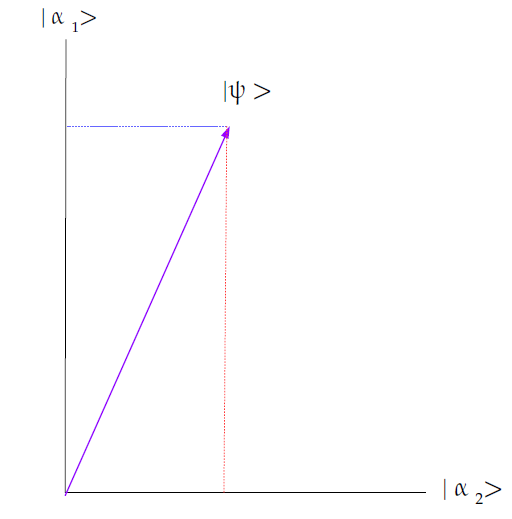
\includegraphics[scale=0.4]{./figures/state}
	\label{statevec}
	\caption{ The quantum state can be abstractly represented as a vector in the state space}
\end{figure}
Since the magnitude of $ | \psi\rangle $ should be $1$, i.e.
\[
| |\psi \rangle | = 1,
\]
any transformation made upon this ket is ought to a rotation in the state space. If that space is quantised, the rotation is only possible in  integer multiples , and via a ladder ( raising and lowering) operators similar to what we have seen in the (orbital) angular momentum. Hence all these internal degrees of freedom are \textbf{physical realisations} of the same mathematical structure discussed earlier in the angular momentum.\\
These facts are very powerful, because it allows us to apply the same techniques, and thought processes to many physical systems ( with  modifications that appears naturally ). Depending on the nature of the physical problem ( the symmetry, the number of degrees of freedom ..etc). To illustrate this power,  this technique ( which is known formally as \textbf{representation theory}) is used extensively in Fundamental physics. The whole standard model of particle physics is fundamentally  built upon the same idea of \textit{representation}, quantum electrodynamics and quantum chromodynamics ..etc
\begin{figure}
	\centering 
	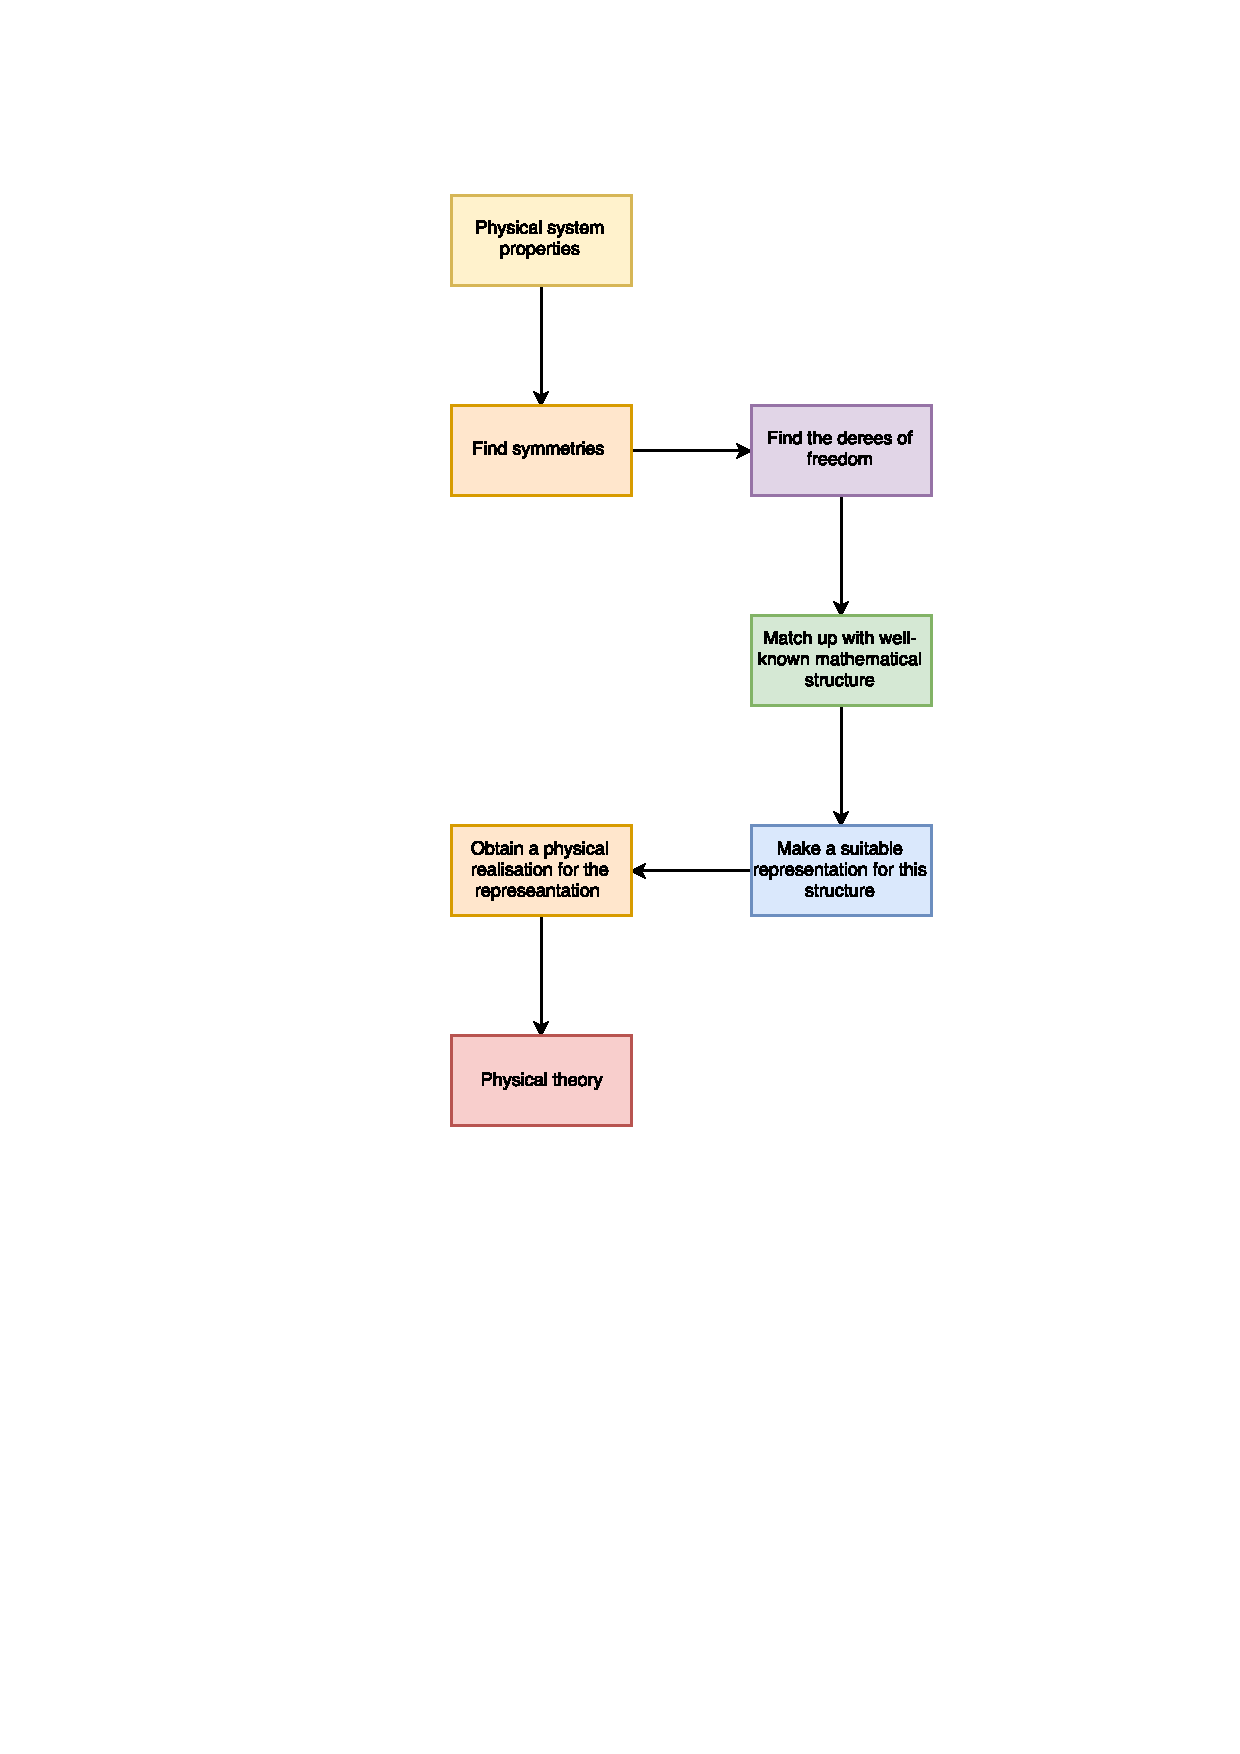
\includegraphics[scale=0.9]{./figures/Rep}
	\label{rep}
	%	
\end{figure}
\section{Discovery of electron's magnetic  dipole moment}
In 1925, the idea of 'spin' angular momentum for electron was first proposed  George Uhlenbeck and Samuel Goudsmit to explain hyperfine splitting in atomic spectra. However, in 1922,  Otto Stern and Walther Gerlach had shown that electrons act  like tiny magnetic bars ( they have a magnetic dipole moment), and that magnetic moment takes particular values only.\\ We are going to construct step-by-step the theory of quantum spin via the observations of S-G experiment, and discuss the mathematical properties of our construction. Following the lead of the philosophy developed above. \\
\par 
S-G apparatus is basically a magnetic field that is free to be in any direction, $x,y,z$. As a beam of electrons is passed through the S-G apparatus, the beam splits either in the positive or negative direction ( say the $B$ field is aligned with the  $z$ axis ). The split is due to a change of energy of the beam, because electron's have magnetic dipole moment, and it takes a $\pm$ values or $ 1/2$ values only, otherwise ... If the electron has an integer multiples of some magnetic dipole moment, not $1/2$ the splitting would be at least in three ways, for $ \pm$ direction  and renaming of the beam passing through unaffected.  Quantitatively we write the change of the energy is given by :

\begin{equation}
\Delta H = \vec \mu \cdot \vec B.
\end{equation}
Since $ \vec B = B_z$ only the  projection of the magnetic dipole moment in the $ z$ direction counts, we hence conclude that :
\begin{equation}
\mu _z  = \pm \frac{1}{2} \; \; \cdot const.
\end{equation}
Same effect is observed if the $B$ field was aligned with any axis not just the $z$ axis. Hence the observable of the dipole magnetic moment is associated with a vector operator  $ \vec  \hat\mu$  that has an eigenvalues of $1/2$ of some constant. This constant was found experimentally, and called the \textbf{Born magnetron} $ \mu_B$ for the electron, but generally it is noted by $ \gamma$ the \textbf{gyromagnetic ratio}, being more careful, Born magnetron and the gyromagnetic ratio are not exactly equal, due to relativistic effects, and Thomas precession $ \gamma = g_s \cdot \mu_B$ where $ g_s$ is \textbf{called Land\'{e} g-factor }. \\ In fact we write :
\begin{equation}
\hat {\vec \mu }= -g_s \mu_B \frac{ \hat {\vec S}}{\hbar}
\end{equation}
We call the operator $ \hat \vec S$ the spin operator .
\section{ Electron's spin}
Although $ \hat \vec S$ does not correspond to a direct observable ( nobody can detect the spin directly separately from the magnetic dipole moment) But seems very natural to study the spin rather than the magnetic dipole moment directly. Although there is no classical analogy to the spin, as electrons do not spin around themselves ( they are dimensionless points ) but spin is a form of angular momentum corresponding to an internal degree of freedom for the electron.\\
So far, from S-G experiment,  we can conclude that :
\begin{equation}
\langle \hat S_z \rangle = \pm \frac{1}{2} \hbar 
\end{equation}
We hall stick with $z$ but any component gives as similar results as the $ S_z$. And the $\hbar$ is just to reserve the dimension of the spin, since it is an angular momentum. We let , for convince denote :
\begin{equation}
\langle \hat S_z \rangle = m_s \; \; \; \;  \; \; \; \; \;\; m_s = -\frac{1}{2} \hbar , +\frac{1}{2} \hbar 
\end{equation} 
 Note how similarities in notation with the orbital angular momentum is appearing. Now, we turn into studying the spin operators more, via repeating the S-G experiment in the following way:\\
Start with S-G apparatus in the $z$ direction, take the half of the initial beam that is aligned in the $+z$ direction ( having $m_s = +1/2 \hbar$) passed though another S-G apparatus but aligned in the $x$ direction, it shall split the beam once again. This time in the $\pm x$ directions. One would expect that by these two apparatuses; we were able to measure two observables associated with $ \hat S_z$ and  $\hat S_x$. Nevertheless, experiments have shown that this is not true, as taking the $1/4$ of the beam that passed via the $+z$ first and $+x$ second, to a third S-G apparatus aligned in the $z$. We expect only one beam to pass in the $+z$ direction, but this doe not happen. The beam splits into two a third time ! This does not happen if we passed it ( initially) into three consecutive S-G apparatuses aligned in the $z$ direction. Hence, we cannot measure the spin in to direction simultaneously. This is mathematically written as   :
\begin{equation}
[ \hat S_z,\hat S_x] \neq 0
\end{equation}
In fact the commutation relation for the spin operators take the form  for the indices $ i,j,k$ taking the values $ x,y,z$:
\begin{equation}
[ \hat S_i\hat S_j] = i \hbar \epsilon_{ij}^k \hat S_k
\end{equation}
\footnote{The symbol $\epsilon_{ij}^k $ is called the Levi-Civita symbol and it is equal to $0$ if $i=j$ and $+1$ for even permutation and $-1$ for odd permutations of the indices }
Which is the same as for the $\hat L$'s that we studied before.  We can therefore, adopting the philosophy of previous lectures define the following operators:
\begin{equation}
\hat S_\pm = \hat S_x \pm i \hat S_y
\end{equation}
and:
\begin{equation}
\hat S^2= \hat S_x ^2 +\hat S_y ^2+\hat S_z ^2
\end{equation}
With the eigenstates :
\begin{equation}
| s, m_s\rangle
\end{equation}
But the eigenvalue $s$ take one value only $ s= \frac{1}{2} \hbar$ and $ m_s$ as we have seen takes the values $m_s = \frac{\pm1}{2} \hbar $ :
\begin{equation}
\begin{matrix}
\hat S_z | s,m_s\rangle = m_s \hbar |s,m_s\rangle \\ \hat S | s,m_s\rangle = \hbar \sqrt{s(s+1)}|s,m_s\rangle
\end{matrix}
\end{equation}
And the ladder operator \footnote{These operators are a direct result from the quantisation of the spin space }:
\begin{equation}
\hat S_\pm |s,m_{s}\rangle = \hbar\sqrt{s(s+1)-m_{s}(m_{s}\pm 1)} |s,m_{s}\pm 1 \rangle
\end{equation}
The three operators $ \hat S_\pm $ and $ \hat S_z$ form the well-known $su(2)$ algebra commutation relations:
\begin{equation}
\begin{matrix}
[\hat S_\pm , \hat S_z] = \mp \hbar \hat S_\pm \\
[\hat S_+ , \hat S_-] = 2 \hbar \hat S_z
\end{matrix}
\end{equation}
The Hilbert space for the spin is very simple, as it is 2-D only spanned by the basis $ | \frac{1}{2}, +\frac{1}{2} \rangle , | \frac{1}{2}, -\frac{1}{2} \rangle$ or denoted by $ |\chi_+\rangle, |\chi_-\rangle\rangle$, respectively.
\begin{equation}
| \psi \rangle = \sum _{ \lambda = \pm} \alpha_ \lambda |\chi_\lambda\rangle
\end{equation}
representing a superposition of the spin states. 
\section{Infel-van der Warden Symbols}
Not always we can have the luxury of selecting the Cartesian coordinates in order to study the spin alignment, sometimes we need to work with any suitable set of coordinates ( cylindrical, spherical \dots ) . Hence we need to link the spin operator vector to a more mathematically-rigorous argument other than the observations made from S-G experiment.\\
In fact, we may write the spin operator vector $\hat{\vec S}$ in terms of a set of symbols, known as  \textbf{Infel-van der Warden Symbols} \marginpar { Usually Infel-van der Warden Symbols used in advanced texts differ from our notation by the factor of $i$, i.e. they usualy call $ i \sigma^i$ as the symbol} ( $ \sigma ^1, \sigma^2, \sigma^3$ ):
\begin{equation}
\hat{\vec S} = \frac{\hbar}{2} \vec \sigma
\end{equation}
Where, $ \vec \sigma = ( \sigma ^1, \sigma^2, \sigma^3 )$ is called the \textbf{Pauli vector }, and these symbols are known in the physics literature as \textbf{Pauli spin matrices }, Due to their relation - in this context- with the spin operator. \\
It goes without saying that the spin operators really have inherited the mathematical properties ( commutation relations) from the Infel-van der Warden Symbols, or -as we shall call them from now on- the Pauli spin matrices. So, naturally there exist the two symbols:
\begin{equation}
\sigma ^{\pm} = \sigma^1 \pm i \sigma ^2
\end{equation}
That along with $ \sigma^3$ form the $su(2)$ algebra commutation relations:
\begin{equation}
\begin{matrix}
[\sigma^3,\sigma^{\pm}] = \pm i \sigma^\pm \\
[ \sigma^+, \sigma ^-] = i \sigma^3
\end{matrix}
\end{equation}
Also note that $$ [\sigma^i, \sigma^j] = 2 i \varepsilon^{ij}_k\,\sigma^k $$ 
Moreover, the pauli spin matrices have an important mathematical property called the \textbf{Clifford algebra }relation:
\begin{equation}
\{\sigma^i, \sigma^j\} = \sigma^i \sigma^j + \sigma^j\sigma^i = 2 \delta ^{ij}
\end{equation}
We call the operation $ \{ \cdot,\cdot\}$ the \textbf{anticommutator}. From this property we can easily prove that:
\begin{equation}
(\sigma^1) ^2 = (\sigma^2) ^2 = (\sigma^3) ^2 = \delta ^{ij}
\end{equation}
\par 
So far, we only dealt with \textit{abstract}, mathematical entities, and their properties (commutation relations), In order to use them in physical calculations, we need to find a proper \textbf{representation} for them in order to be realised in the physical world. We shall find that there are many possible representations for the Pauli spin matrices, that have a direct physical application and meaning. In fact, spin of the electron is only a simple application of the representations for the Pauli spin matrices, others go as deep as the \textit{electroweak interaction } in the standard model of particle physics, and supersymmetry! However, there are other representations, that seems to be of an interest of mathematicians mainly like the quaternions (a higher form of complex numbers that has 3 imaginary units)  .
\section{Matrix representation of spin states}
In the last sections, we have introduced the spin operators and their eigenstates. We discovered the algebra of spin operators, and derived the Pauli spin matrices. However, we only stated their properties abstractly without defining a particular representation for them, now we aim to realise the spin algebra in a simple representation. \\ Consider the eigenkets $ | \chi_-\rangle$ and $ | \chi_+\rangle$.They form a basis for a 2-D Hilbert space of the internal degree of freedom, we have called the ` spin' . It is natural to introduce a canonical representation for these kets as the column vectors :
\begin{align}
| \chi_+\rangle \equiv \begin{pmatrix}
1\\0
\end{pmatrix} \\
| \chi_-\rangle \equiv \begin{pmatrix}
0\\1
\end{pmatrix}
\end{align}
Now, the action of the spin operators $ \hat S_1 , \hat S_2, \hat S_3$ and the ladder spin operators $\hat S_+ , \hat S_-$ on the kets is :
\begin{align}
\hat S_1 | \chi_\pm\rangle &= \frac{\hbar}{2} | \chi_\mp\rangle & \hat S_2 | \chi_\pm\rangle &= \pm i\frac{\hbar}{2} | \chi_\mp\rangle & \hat S_3 | \chi_\pm\rangle &=\pm \frac{\hbar}{2} | \chi_\pm\rangle  \nonumber\\
\hat S_\pm | \chi_\mp\rangle &=  \hbar | \chi_\pm\rangle & & &\hat S_\pm | \chi_\pm\rangle &=  0
\end{align}
We can easily express the operators above as matrices, and with the help of the identity:
\begin{equation}
\vec S = \frac{\hbar}{2} \vec \sigma
\end{equation}
We may write the explicit expression of the Pauli matrices:
\begin{align*}
\sigma_ 1  &=
\begin{pmatrix}
0&1\\
1&0
\end{pmatrix} \\
\sigma_2  &=
\begin{pmatrix}
0&-i\\
i&0
\end{pmatrix} \\
\sigma_ 3  &=
\begin{pmatrix}
1&0\\
0&-1
\end{pmatrix} \,.
\end{align*}
And:
\begin{align*}
\sigma_+ =\begin{pmatrix}
0&1\\
0&0
\end{pmatrix}\\
\sigma_- =\begin{pmatrix}
0&0\\
1&0
\end{pmatrix}
\end{align*}
We shall only deal with the index-down matrices and drop the ket notion on the eigenstate, calling them. For convenience and consistency with quantum mechanics textbooks.\\ Sometimes, the states $ \chi_+ , \chi_-$ are denoted by $ \alpha$ and $\beta$, respectively. The spinor \boldmath${ \chi} $ is defined as:
\begin{equation}
\mbox{\boldmath $\chi$ } = \unboldmath\begin{pmatrix}
\chi_+\\\chi_-
\end{pmatrix}
\end{equation}
Moreover, we can define the Hermitian conjugate of the spinor:
\begin{equation}
\mbox{\boldmath $\chi$ }^\dagger = \unboldmath\begin{pmatrix}
\chi^*_+&\chi^*_-
\end{pmatrix}
\end{equation}
That satisfies:
\begin{equation}
\mbox{\boldmath $\chi$ }^\dagger  \mbox{\boldmath $\chi$ } =\unboldmath 1
\end{equation}
We can calculate the expected value for an operator $ \hat \Omega $ acting on the spin Hilbert space by:
\begin{equation}
\langle\hat \Omega \rangle = \mbox{\boldmath $\chi$ }^\dagger \unboldmath  \hat \Omega   \;	\mbox{\boldmath $\chi$ }
\end{equation}
\section{Geometric representation}
There is another representation for spin, connected to the ` spin vector ' pointing in the 3-D space. In spherical polar coordinates, one may write the spin states as:
\unboldmath
\begin{align}
\unboldmath
\chi_+  &= e^{i\left( \delta- \varphi/2\right) }\;\cos \frac{1}{2} \theta & \chi_+  &= e^{i\left( \delta+ \varphi/2\right) }\;\sin\frac{1}{2}\theta 
\end{align}
Where $ \varphi , \theta$ are the polar and azimuthal angels, respectively and $\delta$ is an arbitrary phase.\\ In order to see why this representation is correct, we start by evaluating the probability of detecting the particle spinning up, w.r.t. the $z$ direction:
\begin{equation}
| \chi_+|^2 = \cos^2 \frac{1}{2}\theta 
\end{equation}
Similarly for the down direction:
\begin{equation}
| \chi_-|^2= 1- \chi_+|^2 =1- \cos^2 \frac{1}{2}\theta = \sin^2 \frac{1}{2}\theta 
\end{equation}
It is clear now, what is the r\^{o}le of the magnitude of the spin states, in terms of $ \theta$. However, we need to discuss further the r\^{o}le that the phase plays. \\ Lets start by calculating the expected values of the spin operators:
\begin{align}
\langle \hat S_x\rangle &= \frac{1}{2} \sin \theta \cos \varphi \nonumber \\
\langle \hat S_y\rangle &= \frac{1}{2} \sin \theta \sin\varphi \\
\langle \hat S_z\rangle &= \frac{1}{2} \cos \theta \nonumber 
\end{align}
Now, assume we wish to rotate the coordinates by an angle $ \gamma$ around $ z$. We have the rotation matrix :
\begin{equation}
R(\gamma) = \begin{pmatrix}
e^ {i \gamma/2} & 0 \\
0&	 e^ {-i \gamma/2} 
\end{pmatrix}
\end{equation}
Applied to the spinor \boldmath$\chi$ is equal to:
\unboldmath
\begin{equation}
R(\gamma)	\mbox{\boldmath $\chi$ } = \unboldmath \begin{pmatrix}
e^ {i(\delta - \frac{1}{2}(\varphi-\gamma))} \cos \frac{1}{2}\theta \\
e^ {i(\delta +\frac{1}{2}(\varphi-\gamma))} \sin \frac{1}{2}\theta
\end{pmatrix}
\end{equation}
Notice that, in order for the spinor to return to its original state, before rotation, one needs not to make a $ 2 \phi$ rotation. Rather a rotation by $ 4\pi$. This is the main characteristic of spinors, that makes them ` very' different from vectors, and manifesting itself in terms of the phase factor in the geometrical representation. Sometimes we denote this characteristic by saying that the ` group' of spin transformations \textbf{double covers} the `group' of spatial transformations.  \\
In order to picture this in a deeper way, one can think of the spinor's internal space as a M\"{o}bius band - illustrated in the figure 1. A vector on the M\"{o}bius band needs to be transported along the band twice, in order to return to its initial state. 
\begin{figure}
	\centering
	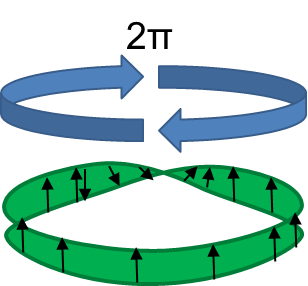
\includegraphics[scale = .8]{./figures/mb}
	\caption{ A spinor transformation can be thought of as a vector on a  M\"{o}bius band.}
\end{figure}
\section{ Spin in constant magnetic field}
A particle with a spin - an electron- for example is put in a constant magnetic filed, such that the direction of the field is parallel to the $z$-component of the spin. The Hamiltonian for such system is given by:
\begin{equation}
H= -\gamma \vec{B}\cdot \vec S
\end{equation}
such that $ \gamma = e/m$, the  ratio between the electron's charge and its mass.And $ \vec B \cdot \vec S = B S_z$.\\
It is clear that:
\begin{equation}
[ H, S_z] =0
\end{equation}
Implying that there exist  eigenstates for $H$ and $S$ simultaneously. Since we already know the eigenstates for $S_z$,  and represented by the spinor $ \chi$ . We then write :
\begin{equation}
H \chi = E \chi 
\end{equation}
or:
\begin{equation}
- \gamma B \, S_z \chi = E \chi .
\end{equation}
Since, $ S_z \chi = \pm \frac{1}{2} \hbar \chi$	 The eigenenergies are:
\begin{equation}
E_{\pm} = \mp \mu_B B
\end{equation}
The constant $ \mu_B = \frac{e \hbar}{2 m_e}$ is Born magneton. It is necessary to add another constant $g_s$ as we have seen earlier to this equation, known as the Land\'{e} g-factor, because the electron \textit{precesses} in the magnetic field. We then have:
\begin{equation}
E_\pm = \mp g_s \mu_B B
\end{equation}
\subsection{ Stationary states}
Since we have found the energy spectrum for an electron in magnetic field, we may now write the time evolution of the state $ \chi$, using the equation:
\begin{equation}
\chi (t) = e^{-i \omega t} \chi(0)
\end{equation}
We have then, for $A$ and $B$ are normalisation constants:
\begin{equation}
\chi(t) = A e^{-i \omega t} \chi_+ + B e^{i\omega t} \chi_-
\end{equation}
or:
\begin{equation}
\chi (t) = A e^{i \frac{1}{2} \gamma Bt} \begin{pmatrix}
1\\0
\end{pmatrix}
+  B e^{-i \frac{1}{2} \gamma Bt} \begin{pmatrix}
0\\1
\end{pmatrix} = \begin{pmatrix}
A e^{i \frac{1}{2} \gamma Bt} \\ B e^{-i \frac{1}{2} \gamma Bt}
\end{pmatrix}
\end{equation}
\section{Electron paramagnetic resonance EPR}
From the above analysis, we have learnt that an electron in a magnetic field could occupy one of two energy states, depending on $m_s$ :
\begin{equation}
E_{m_s} = m_s g_s \mu_B B
\end{equation}
\begin{figure}
	\centering
	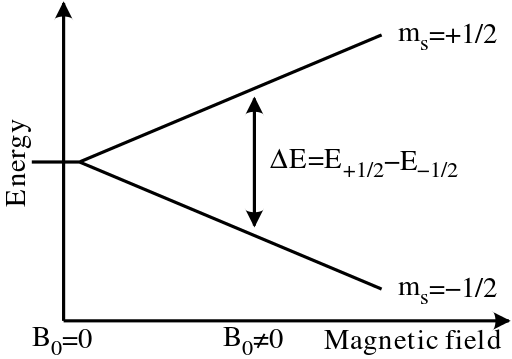
\includegraphics[scale = .4]{./figures/epr}
	\caption{Energy states of electron in a magnetic field $B$.}
\end{figure}
\begin{figure}[h!]
	\centering
	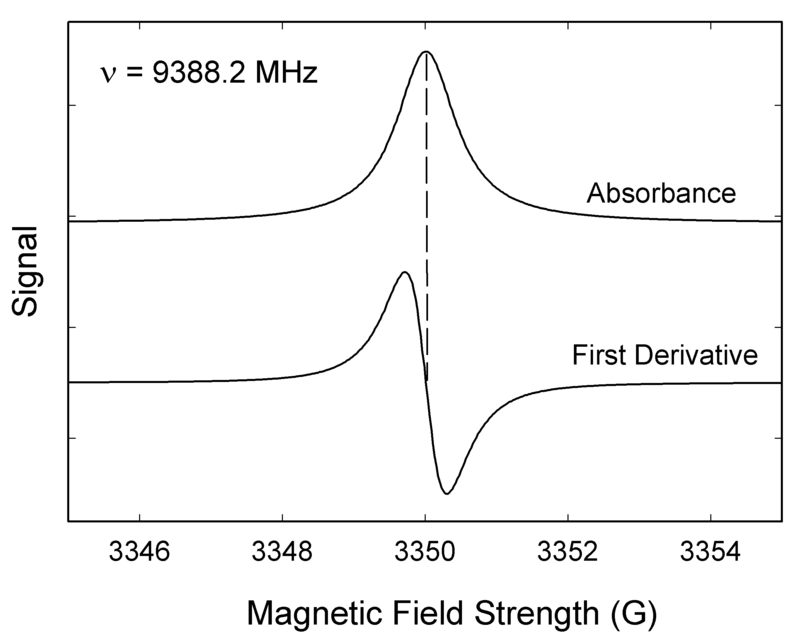
\includegraphics[scale = .3]{./figures/eprlines}
	\caption{EPR absorption resonance for $ \nu=9388.3 MHz$}
\end{figure}
A transition from one energy state to another, is obtained by absorption / emission of photon of energy equal to $ \Delta E = g_s \mu_B B$ :
\begin{equation}
h \nu_r = g_s \mu_B B
\end{equation}
If an ensemble of electrons in the magnetic field is exposed to photons of frequency $ \nu= nu_r$, then the electrons shall absorb them, otherwise no absorption will occur -only elastic scattering-. This peak of absorption is known as\textbf{ electron paramagnetic resonance} or $EPR$. Moreover, $ \nu_r$ is known as the resonance frequency. 

This phenomena is very important in may areas , like measuring the value of the $ g$ factor, and detecting \textit{free radicals} in biological systems.\\
In order to understand the reason for detecting absorption lines rather than the emission lines in EPR, we turn to calculating the population of electrons in the upper energy level $ n_{upper}$ and the lower level $ n_{lower}$, using Maxwell-Boltzmann statistics, under a thermodynamic temperature $T$ :
\begin{equation}
\frac{ n_\text{upper} }{ n_\text{lower} } = \exp{ \left( -\frac{ E_\text{upper}-E_\text{lower} }{ kT } \right) } = \exp{ \left( -\frac{ \Delta E }{ kT }  \right) } = \exp{ \left( -\frac{ h\nu_r }{ kT }\right) }
\end{equation}
Where $k$ is Boltzmann constant .\\
We observe that at room temperature $ T \sim 300 K$ and typical microwave frequency  $ \nu_r \sim 9.7 GHz$ the ratio is about $ n_{upper}/n_{lower} \approx0.998$. That means the upper population is slightly less than the lower one, implying transitions from the lower to upper energy states is more probable than the reverse transitions. 
\section{Problems}
\begin{enumerate}
	\item Show that for Spin vector $ \vec S$, the  vector product with itself is equal o
	\[ \vec S \wedge \vec S = i \hbar \vec S \]
	\textit{hint: use the expression for the vector product} $ \vec S \wedge \vec S  = \varepsilon _{ij} ^k S_i S_j \vec e_k $
	\item prove that $ ( \sigma ^i)^2 = \delta{ij}$
	\item We denote the hermitian Pauli matrix by $  \sigma_i$ , show that it is in fact equal to $ \sigma ^i$. 
	\item Show that, $$ \sigma ^i \; \sigma^j = \delta ^{ij} + i \epsilon_k ^{ij} \sigma ^k$$.
	hint: use both the Clifford algebra and commutation relations the Pauli matrices obey.
	\item Are Pauli matrices unitary ??
	\item What is the action of $ \sigma ^\pm , \sigma ^3$ of the states $ | \chi_\pm\rangle$ ?
	\item Use the definition of the spin vector in terms of the Pauli matrices to prove that $$ \langle \hat S ^2 \ \rangle = \frac{3}{4} \hbar^2$$
	\item Given a vector $ \vec a$, find the dot product: $$ \vec a \cdot \vec \sigma $$ 
	\item Prove that :
	\[ \det ( \sigma ^i) =1 \]
	\item We define the Dirac gamma matrices as :
	\[ \gamma ^k = \begin{pmatrix}
	0&-i\sigma ^k\\i\sigma^k&0
	\end{pmatrix} \]
	Show that the Clifford algebra relation also holds for the gamma matrices :
	\[ \{ \gamma^i, \gamma^j\} = 2 \delta ^{ij} I \]
	\item Given the following $ 2 \times 2$ matrices :
	\begin{align*}
	\sigma_1   &=
	\begin{pmatrix}
	0&1\\
	1&0
	\end{pmatrix} \\
	\sigma_2   &=
	\begin{pmatrix}
	0&-i\\
	i&0
	\end{pmatrix} \\
	\sigma_3  &=
	\begin{pmatrix}
	1&0\\
	0&-1
	\end{pmatrix} \,.
	\end{align*}
	Find their eigenvalues and eigenvectors
	They form the matrix representation for the Pauli spin matrices, moreover, the results obtained will form the explicit expression of the eigenstates $ | \chi_\pm\rangle$ in column form. 
	\item Given 
	\[ \hat \Omega = \begin{pmatrix}
	-1& -i\\ i&2
	\end{pmatrix} \]
	an operator acting on the spin Hilbert space:
	\begin{enumerate}
		\item  Show that it could correspond to an observable.
		\item Decompose it in terms of the Pauli spin matrices.
		\item Find its eigenvalues.
		\item Compute $\langle \Omega \rangle $.
	\end{enumerate}
	\item Since the spin operator is a vector in the 3-D space. Show that if it is rotated by an angle $ \gamma$ around the $z$-axis, the commutation relations algebra remains invariant, for the rotated operator .
	\item Calculate the EPR frequency for an experiment with $B = 100$ Gau\ss{}. where $ \mu_B= 9.274 \times 10^ {-24}$ Joule/Tesla. and the material used is Holmium with  $g_s =1.97$. 
\end{enumerate}